\documentclass[12pt, a4paper]{article}
\usepackage{scrextend}
\usepackage{titlesec}
\usepackage{graphicx}
\usepackage{amsmath}
\usepackage{amsfonts} % for the real number symbol
\usepackage{geometry}
\usepackage[unicode]{hyperref}
\usepackage{titlesec}
\usepackage{titletoc}
\usepackage[sorting=none]{biblatex}
\usepackage{xurl}
\usepackage{enumitem}
\usepackage{indentfirst}
\numberwithin{equation}{section} % number equations by section
\renewcommand{\figurename}{Att.}
\renewcommand{\contentsname}{Saturs}
\renewcommand{\labelenumi}{\arabic{enumi})} % lists with 1)
\setlist{nosep}
\parindent=1cm
\linespread{1.213} % equivalent to 1.5 in word, experimentally.
\addbibresource{refs.bib}

\geometry{
    a4paper,
    lmargin=30mm,
    rmargin=20mm,
    tmargin=20mm,
    bmargin=20mm
}


\titleformat{\section}
    {\normalfont\large\bfseries}{\thesection . }{0.2em}{\MakeUppercase}
\titleformat{\subsection}
    {\normalfont\large\bfseries}{\thesubsection . }{0.2em}{}
\titleformat{\subsubsection}
    {\normalfont\normalsize\bfseries\itshape}{\thesubsubsection . }{0.2em}{}
\titlespacing*{\subsubsection}{0pt}{6pt}{0pt}

\begin{document}
\begin{titlepage}
    \begin{center}
        \vspace*{3cm}
        
        LATVIJAS UNIVERSITĀTE

        DATORIKAS FAKULTĀTE

        \vspace*{4cm}

        \large\textbf{COVID-19 IEROBEŽOŠANAS PROJEKTU PĀRVALDĪBAS ASPEKTI}
        
        \vspace{2cm}
        \normalsize{REFERĀTS IT PROJEKTU PĀRVALDĪBĀ}
         
             
    \end{center}
    \vspace{3cm}
    \begin{addmargin}[18em]{0em}
    Autors: \textbf{Pēteris Račinskis}
    \end{addmargin}

    \begin{addmargin}[18em]{0em}
    \hspace{1cm} Stud. apl. Nr. pr20015
    \end{addmargin}

         
    \vfill
    \begin{center}
    RĪGA 2022
    \end{center}
 \end{titlepage}
\newpage
\tableofcontents
\thispagestyle{empty}
\newpage
\setcounter{page}{3}


\section{Ievads}

Pagājuši nedaudz vairāk kā trīs gadi, kopš parādījās pirmās ziņas, ka Uhaņā --- vienām no Ķīnas lielākajām pilsētām --- dažiem pacientiem konstatēta saslimšana ar iepriekš neredzētu infekcijas slimību. Tās simptomi atgādina gripu, taču vīruss nepieder pie gripas vīrusu dzimtes --- tas ir jauns, potenciāli ārkārtīgi lipīgs koronavīruss. Iepriekšējā reize, kad Ķīnā atklāts cilvēkam bīstams koronavīruss, bijusi 2002. gada rudenī, kad sākusies nāvējošā, taču mērogā samērā ierobežotā SARS epidēmija. Sociālajos tīklos šīs ziņas strauji sasniedz visu pasauli, medicīnas aprindās virmo satraukums, taču rietumos plašsaziņas līdzekļi un sabiedrība kopumā lielu uzmanību tām nepievērš --- jaunu, bīstamu vīrusu parādīšanās kaut kur tālu prom ir regulāra parādība, kas, par spīti dažādu pasaules gala solītāju vaimanāšanai, nekad taču pie nopietnām sekām šeit pie mums nenovedīs. 

Reti kurš toreiz, ap 2019/2020. gadu miju spēja iztēloties to, ka tikai dažus mēnešus vēlāk lielveikalu plauktus panikā tukšos ar tualetes papīru apkrāvušos cilvēku drūzmas un ziņas par miljonu nāvi būs vien fona troksnis, bet šobrīd --- 3 gadus vēlāk --- sadzīvošana ar epidemioloģiskajiem ierobežojumiem ir kļuvusi par ikdienu, vakcinācija --- par karstāko tematu politikā --- un grūti vairs atcerēties, kā dzīve norita pirms tam. Teikt, ka pēdējie daži gadi ir bijuši visnotaļ interesanti valdībām un nevalstiskajām institūcijām, kuru uzdevumis bijis novērst, ierobežot un pārvarēt pandēmijas sekas, būtu maigi. Krīzes vadības stratēģijas un plāni, kas desmitgadēm ilgi bijušas vien teorētiski domas lidojumi, izvilktas no atvilknēm un liktas lietā. Iepriekš neredzēti investīciju apjomi ieguldīti tradicionāli ļoti lēno medicīnas izstrādes un sertificēšanas procesu paātrināšanā. Nācies praktiski saskarties un dārgi maksāt par nevīžīgi veidotiem sabiedriskās domas procesiem. 

Kaut gan pandēmija vēl nebūt nav galā, pagājis pietiekami ilgs laiks, lai varētu pakāpties soli atpakaļ, atskatīties uz šo īpatnējo vēstures periodu un mēģināt izdarīt kādus spriedumus. Kas īsti tika darīts? Kāpēc? Vai izdevās?


\subsection{Referāta mērķis un struktūra}

Šī referāta mērķis ir identificēt un novērtēt nozīmīgākos COVID-19 pandēmijas izplatības ierobežošanas un seku apkarošanas ietvaros veiktos projektus, galvenokārt no suverēnu valstu valdību vai supranacionālu organizāciju skatapunkta. Tā kā šī krīze ir skārusi visu pasauli, ļoti daudzas un dažādas institūcijas ir bijušas iesaistītas šajā procesā. Pie tam faktiski nevienai nav iespējams visu periodu un visas veiktās darbības loģiski apvienot viena projekta ietvaros --- lai veiktu jebkādu analīzi nedrīkst ignorēt faktu, ka jebkuras institūcijas cīņa ar pandēmiju bijusi savstarpēji saistītu, bet atšķiramu projektu virkne. Nākamajā nodaļā tiek aprakstīts, pēc kāda principa nolemts izšķirt dažādus projektus, un kāpēc no ļoti daudzajiem sīkākai iztirzāšanai izvēlēti tieši tie, par kuriem runāts zemāk. Noslēgumā tiek apvienotas gūtās atziņas, izteikti subjektīvi novērtējumi un spriests par lietām, ko būtu bijis iespējams darīt labāk.

\newpage
\section{COVID-19 ierobežošanas projekti}

\subsection{Projektu dalījums un izvēle}

Lai būtu iespējams uz kādu darbību kopumu skatīties no projektu pārvaldības skatapunkta, nepieciešams vispirms saprast, kā tas iederas projekta jēdzienā. Atceroties semestra gaitā izstudētās ``\textit{Project Management Book}'' ievadā sniegto definīciju \cite{proj_book_intro} un nedaudz pārfrāzējot, projektu var definēt kā darbību ar sekojošajām īpašībām:

\begin{enumerate}
    \item tā ir vienreizēja un izpildāma noteiktā laikā --- ja kaut kas tiek darīts daudzkārt vai atkārtots nebeidzami, tas jau ir process. Procesa ieviešana ir projekts, bet ne pats process;
    \item tai ir skaidri definēts sākums un noslēgums;
    \item no tās tiek sagaidīts konkrēts rezultāts --- sasniegts mērķis;
    \item tai piešķirti konkrēti resursi;
    \item tās izpildi vada skaidri definēta projekta vadības hierarhija. 
\end{enumerate}

Tātad pilnīgi patvaļīgi izvēlēties kādu tematu un sākt tam piemērot projektu vadības terminoloģiju nav pareizi. Pandēmijas apkarošana ir ļoti garš un kopumā nestrukturēts process. Pat ja izvēlamies kādu konkrētu organizāciju --- piemēram, Latvijas Republikas Ministru kabinetu --- nav iespējams definēt vienotu mērķi, resursus, vadības hierarhiju vai noslēguma nosacījumus visam šim procesam kopumā. Tāpēc jāievieš smalkāks un precīzāks dalījums apakšuzdevumos, kuriem visas projekta īpašības var piemērot.

Viena no pirmajām un sabiedrības prātos vispamanāmākajām darbībām, ko pasaules valstu valdības realizējušas, ir vīrusa izplatības ātruma samazināšanas līdzekļu pieņem-šana. Tas ticis darīts jau pašā laika posma sākumā, kad par slimību vēl bijis zināms visnotaļ maz, pieejamas bijušas tikai ļoti trulas un invazīvas metodes, kuru efektivitāte --- tikai aptuveni aplēšama. Lai tās varētu izteikt kā projektus, nepieciešams katru ārkārtas ierobežojumu ieviešanas stadiju --- reakciju uz augošas saslimstības ``vilni'' --- izdalīt atsevišķi. Tas ne vienmēr ir vienkārši, jo pastāvējušas dažādas pakāpeniskas ierobežojumu pastiprināšanas sistēmas, turklāt katra perioda noslēguma parasti ne visi pieņemtie līdzekļi ir atcelti. Tomēr kopumā iespējams definēt vismaz aptuvenu mērķi, sākumu un noslēgumu, sagaidāmos un sasniegtos rezultātus kā arī atbildīgo vadības hierarhiju katram pandēmijas vilnim.

Otra tēma, kas interesanta tieši no projektu pārvaldības viedokļa, ir vakcīnas. Šeit gan saskaramies ar sarežģījumu --- pirmajā pandēmijas gadā noritēja faktiski tikai vakcīnu izstrādes un testēšanas procesi, bet pēc tam jau izstrādātās vakcīnas nācies izmantot nepieredzēta apjoma imunizācijas kampaņā. Tā kā šie ir ļoti atšķirīgi uzdevumi ar dažādiem mērķiem un līdzekļiem, nolemts vakcīnu izstrādi un sertifikāciju, kas notikusi pamatā ASV, Ķīnā, Krievijā un ES 2020. gadā, aplūkot atsevišķi no sabiedrības vakcinācijas visur pasaulē 2021. gadā. Tāpat vakcinācija atdalīta no vīrusa izplatības ātruma mazi-nāšanas projektiem, jo, kaut gan tie ir savstarpēji saistīti, vakcinācijai nosprausti mērķi ilgākos termiņos un tā noris paralēli vairākiem ierobežojumu etapiem.

\subsection{Vīrusa izplatības tūlītēja samazināšana}

\subsubsection{Pirmie viļņi --- 2020. gada pavasaris}

\subsubsection{Otrie viļņi --- 2020. gada rudens}

\subsubsection{Vēlāki vilņi, apvienojums ar vakcināciju}

\subsection{Vakcīnu izstrāde, ieviešana}

\subsection{Vakcinācija}


\newpage
\section{Secinājumi}

Literatūras analīzē sniegts īss un nebūt ne pilnīgs --- vai vienlīdzīgi sadalīts --- līdz šim par atdarinošo mašīnmācīšanos veiktās pētnieciskās darbības pārskats. Jau izvēloties, par kurām tēmām rakstīts plašāk, par kurām --- mazāk detalizēti --- iespaidu uz darba saturu ir atstājusi motivējošās problēmas specifika. Tagad nepieciešams pie tās atgriezties un novērtēt, kas no visa nozarē pētītā un izgudrotā attiecas uz darba ievadā aprakstīto uzdevumu --- mešanas kustību iestrādāšanu atkritumu vai citu objektu pārvietošanā.

\subsection{Svarīgākās atziņas}

\begin{figure}[t!]
    \centering
    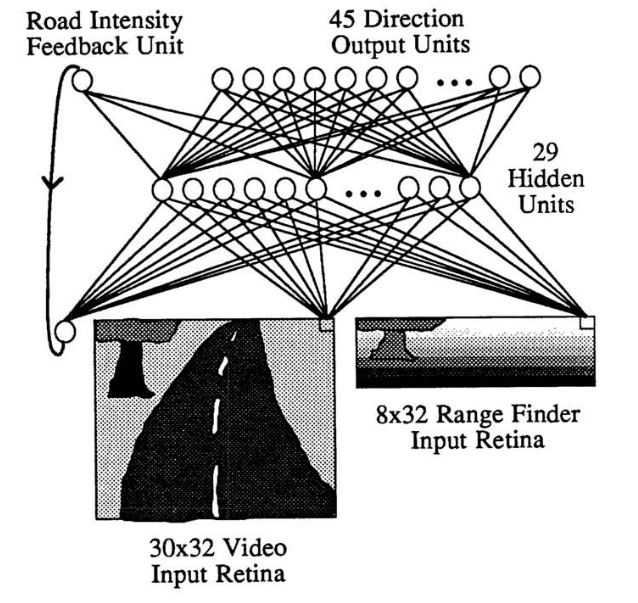
\includegraphics[height=6.8cm,page=1]{../img/alvinn_architecture.png}
    \caption{ALVINN modeļa uzbūve \cite{enc_stim}}
\end{figure}

\newpage
\addcontentsline{toc}{section}{Atsauces}
\printbibliography[title=Atsauces]

\end{document}